\documentclass[12pt]{article}
\newif\ifanswer\answertrue\answerfalse% comment out to show/hide answers
\usepackage{../preamble3}% preamble always after \newif\ifanswer
%\pagenumbering{gobble}
\title{Art Of Problem Solving - AMC 10 \\ Week 7}
\author{Patrick \& James Toche}
\date{July 24, 2021}

\begin{document}
\maketitle
\begin{minipage}{\textwidth}
\begin{abstract}\setlength{\parindent}{0pt}%
Notes on the AMC-10 Course by Art Of Problem Solving (AOPS).
Copyright restrictions may apply. Written for personal use. 
Please report typos and errors over at \url{https://github.com/ptoche/Math/tree/master/aops}. 
\end{abstract}
\end{minipage}

\thispagestyle{empty}
\clearpage


%%%%%%%%%%%%%%%%%%%%%%%%%%%%%%%%%%%%%%%%%%%%%%%%%%%%%%%%%%%%%%%%%%%%%%%%
\subsection*{1.}

\nopagebreak

Rolly wishes to secure his dog with an 8-foot rope to a square shed that is 16 feet on each side. His preliminary drawings are shown.

\nopagebreak

\begin{center}
  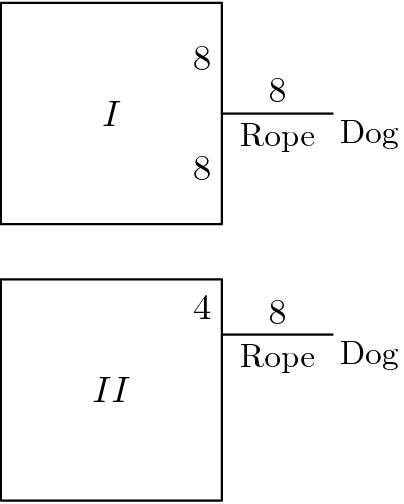
\includegraphics[height=6cm,page=1]{2021-07-24-figure-01}
\end{center}

\nopagebreak

Which of these arrangements gives the dog the greater area to roam, and by how many square feet?

\nopagebreak

\fbox{(A) $I$, by $8\pi$ \quad (B) $I$, by $6\pi$ \quad (C) $II$, by $4\pi$ \quad (D) $II$, by $8\pi$ \quad (E) $II$, by $10\pi$}

\begin{answer}
\begin{center}
  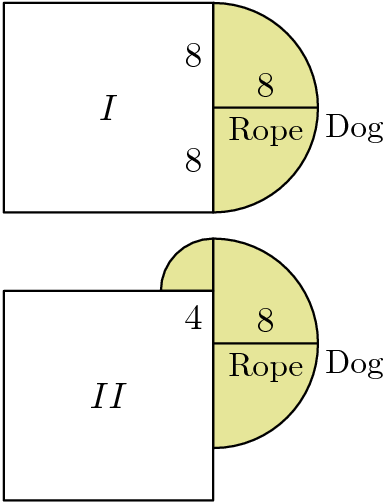
\includegraphics[height=6cm,page=1]{2021-07-24-figure-01b}
\end{center}
\bigskip
Arrangement $I$ gives an area
\begin{align*}
\frac{8^2\,\pi}{2} = 32\pi~\text{ft}^2
\end{align*}
Arrangement $II$ gives a greater area thanks to the ability to turn around the corner of the shed. The added area gives a quarter of a circle with radius $4$. The additional area is: 
\begin{align*}
\frac{4^2\,\pi}{4} = 4\pi~\text{ft}^2
\end{align*}
That is one-eighth more, or $12.5\%$.
\begin{empheq}[box={\mathbox[colback=white]}]{equation*}
    4\pi
\end{empheq} 
\end{answer}
%%%%%%%%%%%%%%%%%%%%%%%%%%%%%%%%%%%%%%%%%%%%%%%%%%%%%%%%%%%%%%%%%%%%%%%%

\iftoggle{showAnswers}{\newpage}

%%%%%%%%%%%%%%%%%%%%%%%%%%%%%%%%%%%%%%%%%%%%%%%%%%%%%%%%%%%%%%%%%%%%%%%%
\subsection*{2.}

\nopagebreak

A square of side length 1 and a circle of radius $\sqrt{3}/3$ share the same center. What is the area inside the circle, but outside the square?

\nopagebreak

\fbox{(A) $\dfrac{\pi}{3}-1$ \quad (B) $\dfrac{2\pi}{9}-\dfrac{\sqrt{3}}{3}$ \quad (C) $\dfrac{\pi}{18}$ \quad (D) $\dfrac{1}{4}$ \quad (E) $\dfrac{2\pi}{9}$}

\begin{answer}
The problem is symmetric along the horizontal and vertical axes, so we can focus on the area denoted $X$ on the figure. Since we know both the side-length of the square and the radius of the circle, we can readily calculate the area of triangle $\trianglehat{OAB}$. Then we calculate the area of the sector $\sectorhat{OAB}$ and subtract $\trianglehat{OAB}$ from it to get $X$. 
\begin{center}
  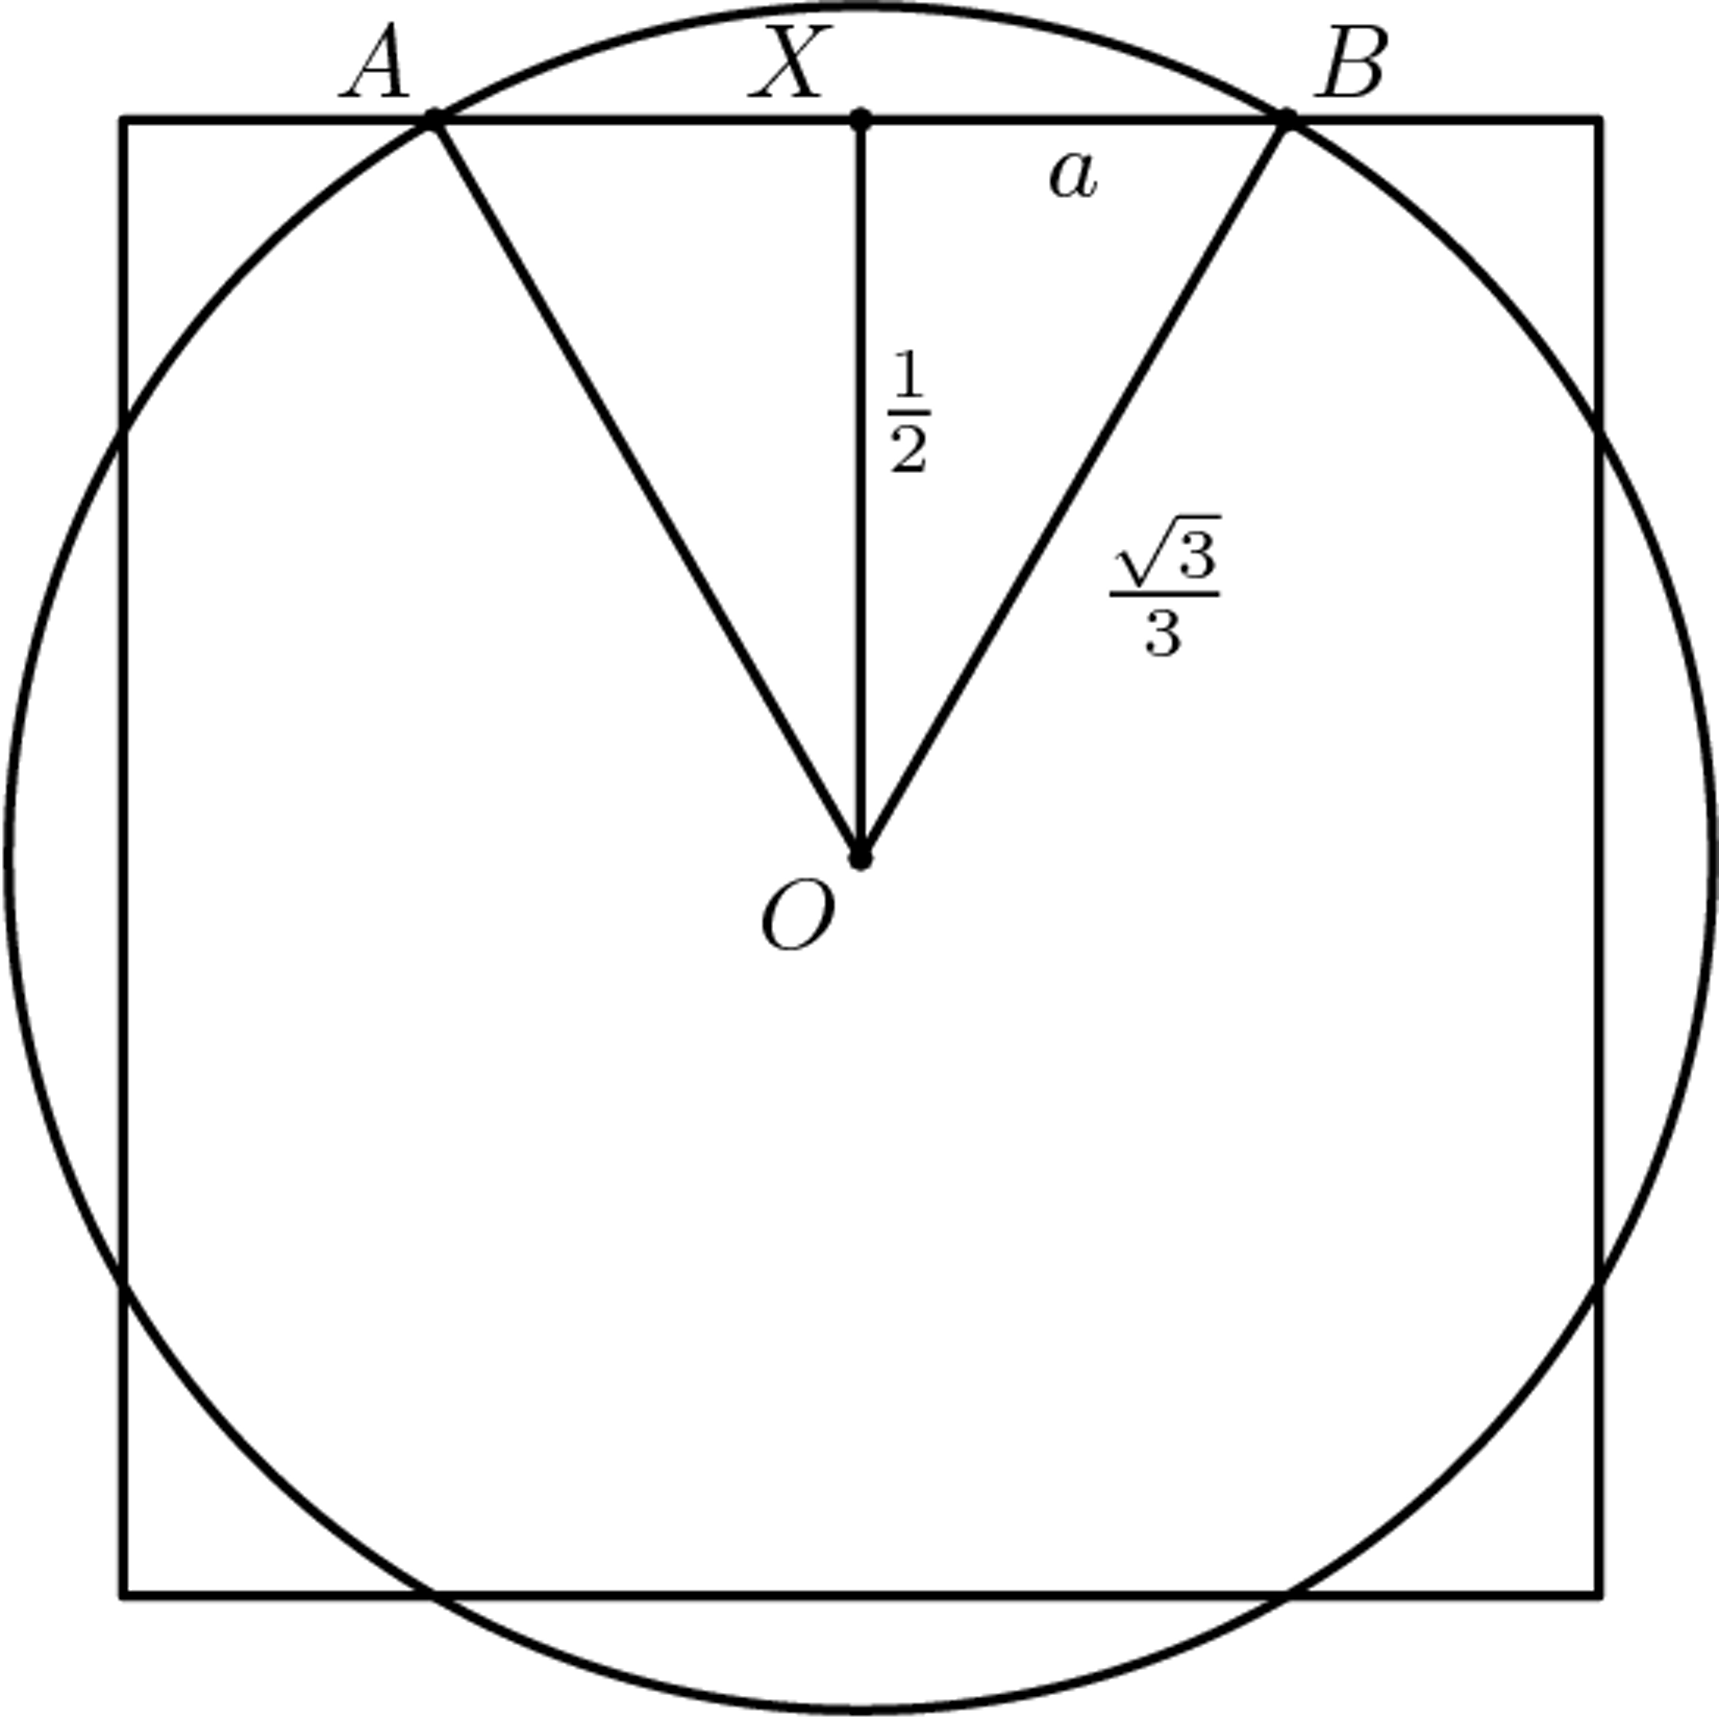
\includegraphics[height=7cm,page=1]{2021-07-24-figure-02}
\end{center}
\bigskip
The area of triangle $\trianglehat{OAB}$ is $a/2$, where 
\begin{align*}
a = \sqrt{\left(\frac{\sqrt{3}}{3}\right)^2 - \left(\frac{1}{2}\right)^2}
  = \frac{\sqrt{3}}{6}
\end{align*}
%Thus,
\begin{align*}
\text{Area of triangle $\trianglehat{OAB}$}~
= \frac{\sqrt{3}}{3}
\end{align*}
and therefore $AB=2a=\sqrt{3}/3=OA=OB$. Triangle $\trianglehat{OAB}$ is an equilateral triangle, implying that the angle of $\sectorhat{OAB}$ is $60^{\circ}$. The area of sector $\sectorhat{OAB}$ is therefore a fraction $60/360$ of the area of the circle:
\begin{align*}
\text{Area of sector $\sectorhat{OAB}$}~
= \left(\frac{60}{360}\right) \pi \left(\frac{\sqrt{3}}{3}\right)^2
= \frac{\pi}{18}
\end{align*}
%And therefore
\begin{align*}
\text{Area of sector $\sectorhat{OAB}$}~
-
\text{Area of triangle $\trianglehat{OAB}$}~
= \frac{\pi}{18} - \frac{\sqrt{3}}{3}
%= \dfrac{2\pi}{9}-\dfrac{\sqrt{3}}{3}
\end{align*}
\begin{empheq}[box={\mathbox[colback=white]}]{equation*}
    \dfrac{2\pi}{9}-\dfrac{\sqrt{3}}{3}
\end{empheq} 
\end{answer}
%%%%%%%%%%%%%%%%%%%%%%%%%%%%%%%%%%%%%%%%%%%%%%%%%%%%%%%%%%%%%%%%%%%%%%%%

\iftoggle{showAnswers}{\newpage}

%%%%%%%%%%%%%%%%%%%%%%%%%%%%%%%%%%%%%%%%%%%%%%%%%%%%%%%%%%%%%%%%%%%%%%%%
\subsection*{3.}

\nopagebreak

Two distinct lines pass through the center of three concentric circles of radii 3, 2, and 1. The area of the shaded region in the diagram is 8/13 of the area of the unshaded region. What is the radian measure of the acute angle formed by the two lines?

\nopagebreak

\begin{center}
  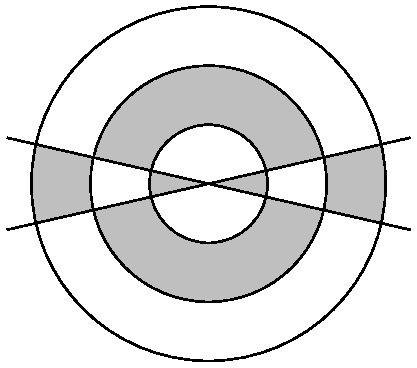
\includegraphics[height=5cm,page=1]{2021-07-24-figure-03}
\end{center}

\nopagebreak

\fbox{(A) $\dfrac{\pi}{8}$ \quad (B) $\dfrac{\pi}{7}$ \quad (C) $\dfrac{\pi}{6}$ \quad (D) $\dfrac{\pi}{5}$ \quad (E) $\dfrac{\pi}{4}$}

\begin{answer}
Let $s$ denote the area of the shaded region and $u$ the unshaded region. Let $\theta$ denote the acute angle formed by the intersection of the two lines. The total area is equal to the area of the larger circle with radius $3$, or $9\pi$, so that $s$ and $u$ satisfy:
\begin{align*}
s + u = 9 \pi
\end{align*}
The ratio of the areas is given by:
\begin{align*}
\frac{s}{u} = \frac{8}{13}
\end{align*}
This is a linear system with solutions $u=\dfrac{39\pi}{7}$ and $s=\dfrac{24\pi}{7}$. 

These areas may also be expressed in terms of $\theta$ by adding up the various sections for each annulus. In general, the intersection of a sector of angle $\theta$ (measured in radians) with an annulus with inner radius $r$ and outer radius $R$ encloses an area of:
\begin{align*}
\frac{\theta}{2\pi} \cdot (R^2-r^2) \pi 
\end{align*}
In particular, the shaded area is:
\begin{align*}
s & = 2 
      \left(  
          \frac{\theta}{2\pi} \cdot 1^2 \pi
        + \frac{\pi-\theta}{2\pi} \cdot (2^2-1^2)\pi
        + \frac{\theta}{2\pi} \cdot (3^2-2^2)\pi
      \right) \\
  & = \theta + 3(\pi-\theta) + 5\theta
    = 3(\pi+\theta)
\end{align*}
Equating the two expressions for $s$ gives:
\begin{align*}
3(\pi+\theta) = \frac{24\pi}{7} 
\implies
       \theta = \frac{\pi}{7}
\end{align*}

\begin{empheq}[box={\mathbox[colback=white]}]{equation*}
    \frac{\pi}{7} ~\text{radians}
\end{empheq} 
\end{answer}
%%%%%%%%%%%%%%%%%%%%%%%%%%%%%%%%%%%%%%%%%%%%%%%%%%%%%%%%%%%%%%%%%%%%%%%%

\iftoggle{showAnswers}{\newpage}

%%%%%%%%%%%%%%%%%%%%%%%%%%%%%%%%%%%%%%%%%%%%%%%%%%%%%%%%%%%%%%%%%%%%%%%%
\subsection*{4.}

\nopagebreak

Many Gothic cathedrals have windows with portions containing a ring of congruent circles that are circumscribed by a larger circle. In the figure shown, the number of smaller circles is four. What is the ratio of the sum of the areas of the four smaller circles to the area of the larger circle?

\nopagebreak

\begin{center}
  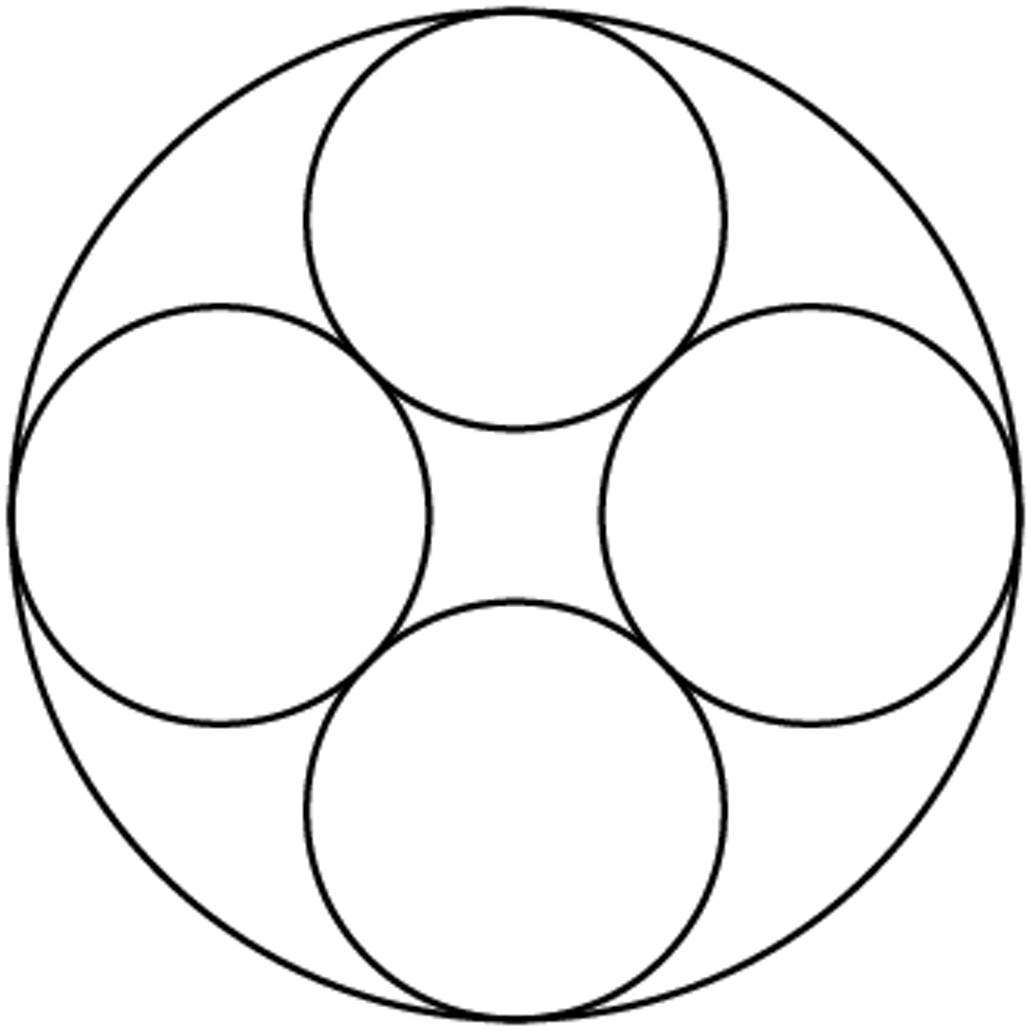
\includegraphics[height=5cm,page=1]{2021-07-24-figure-04}
\end{center}

\nopagebreak

\fbox{(A) $3-2\sqrt{2}$ \quad (B) $2-\sqrt{2}$ \quad (C) $4(3-2\sqrt{2})$ \quad (D) $\dfrac{1}{2}(3-\sqrt{2})$ \quad (E) $2\sqrt{2}-2$}

\begin{answer}
\begin{center}
  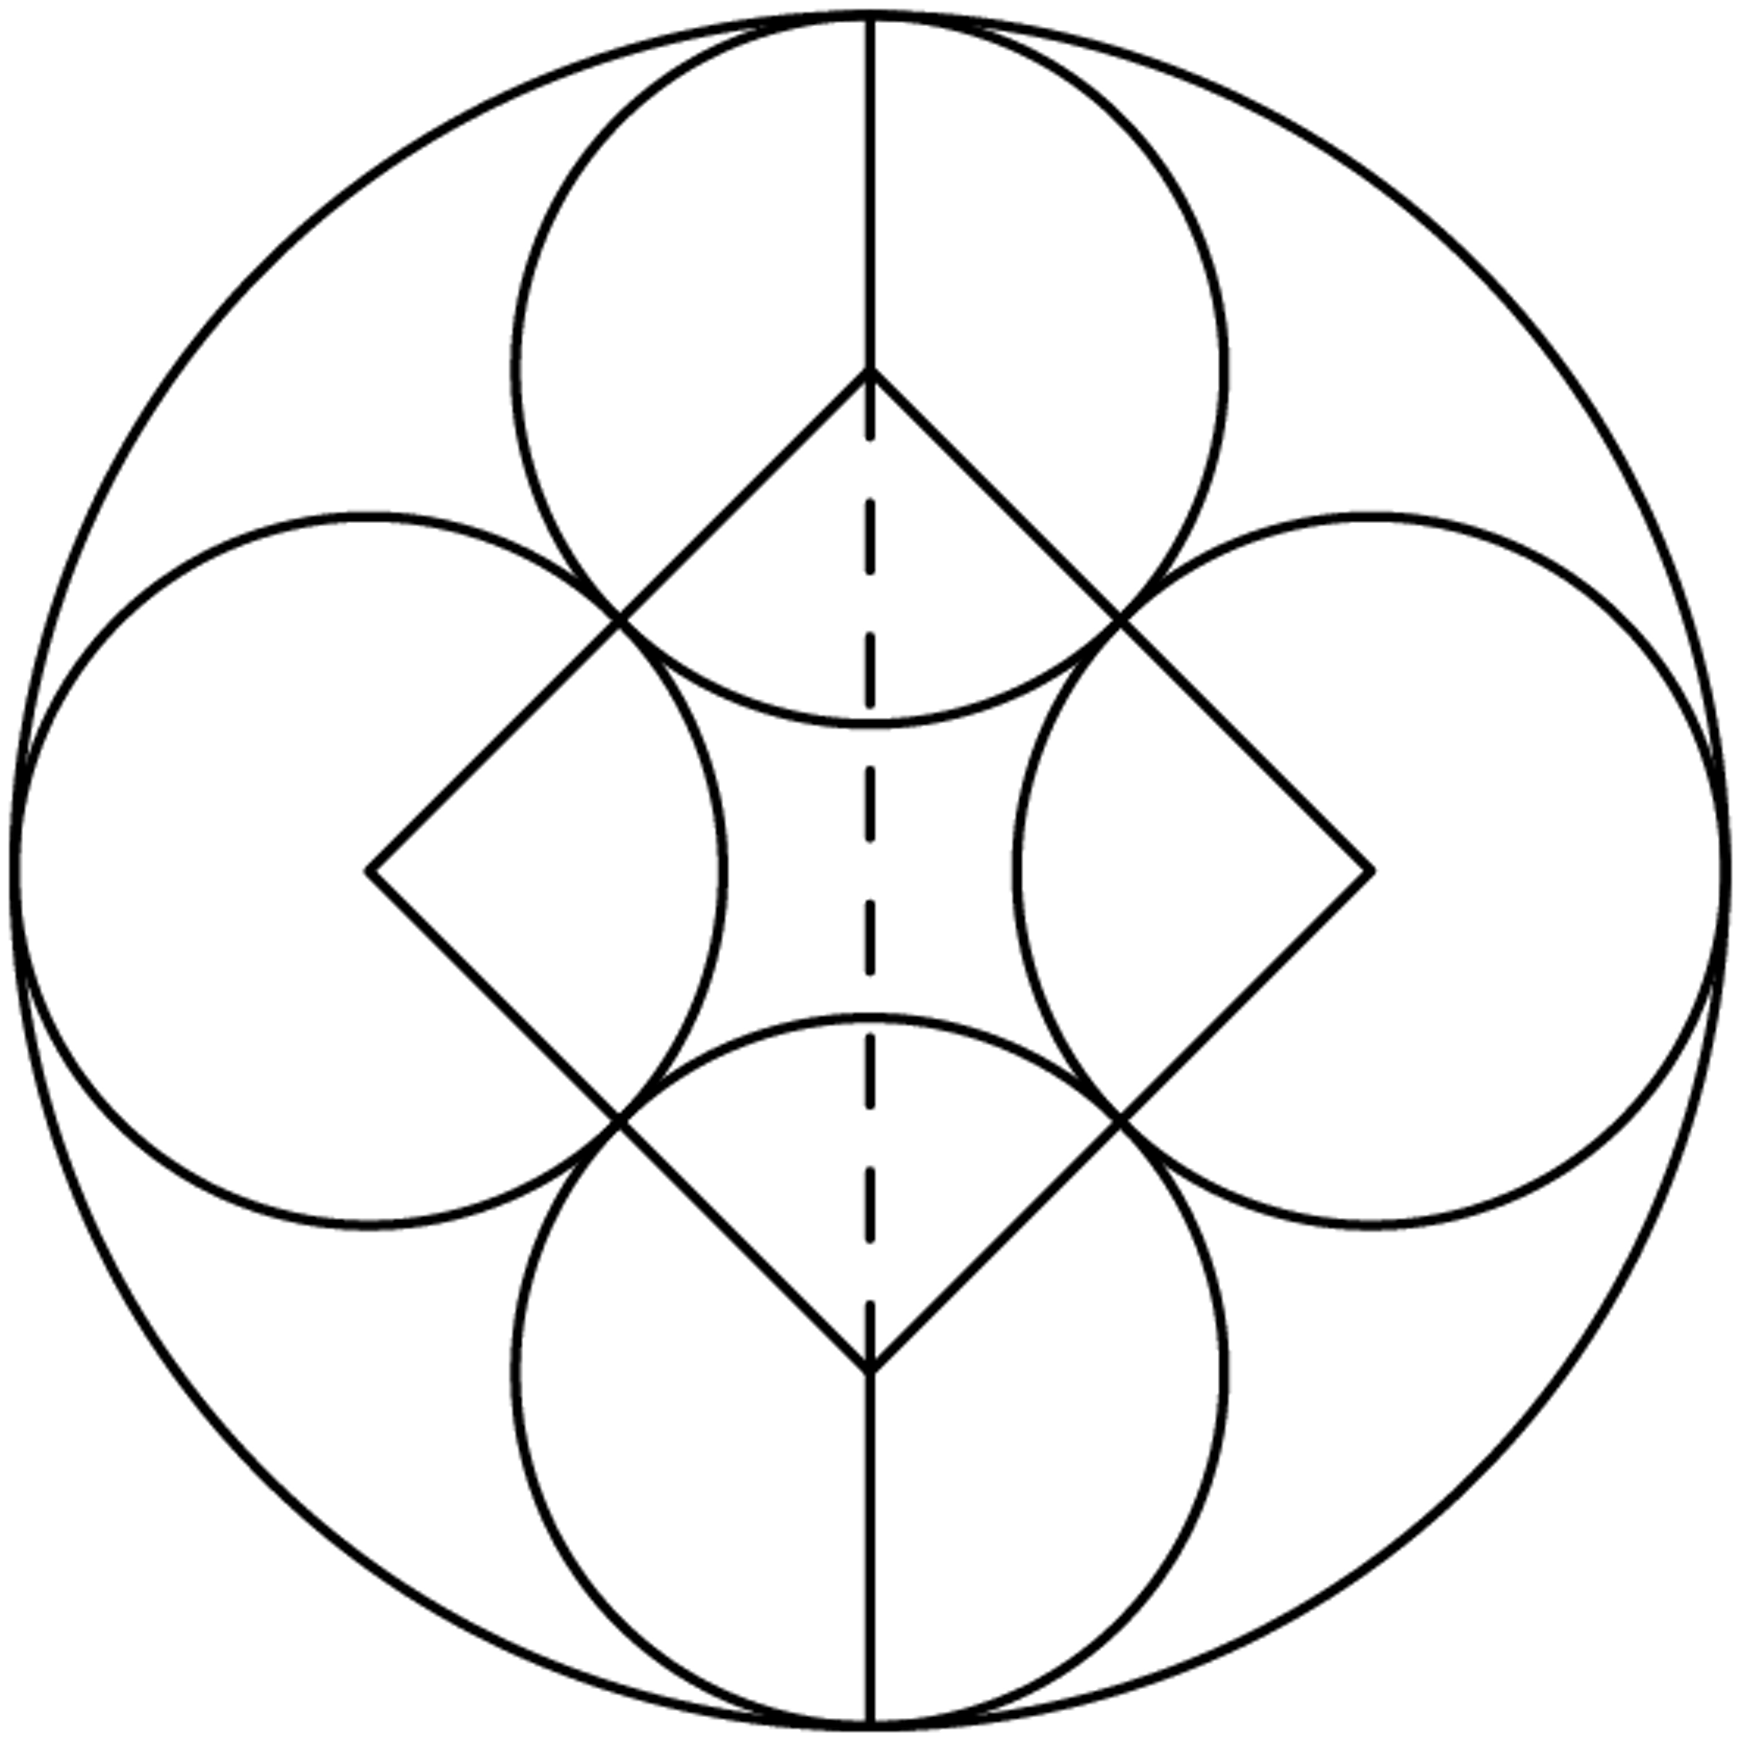
\includegraphics[height=5cm,page=1]{2021-07-24-figure-04b}
\end{center}
\bigskip
Let $r$ denote the radius of a small circle. Since the figure is symmetric along both the horizontal and vertical axes, the four lines connecting the centers of these circles form a square of side length $2r$. The diagonal of these squares is $2r\sqrt{2}$ and therefore the diameter of the large circle is $2r+2r\sqrt{2}$. The area of the large circle is therefore $\pi(1+\sqrt 2)^2r^2 $. The area of the four small circles is $4\pi r^2$. Hence the ratio is:
\begin{align*}
\frac{\text{area of small circles}}{\text{area of large circle}}
  & = \frac{4\pi r^2}{(3+2\sqrt 2)\pi r^2} \\
  & = \frac{4(3-2\sqrt{2})}{(3+2\sqrt{2})(3-2\sqrt{2})} \\
  & = 4(3 - 2\sqrt 2)
    \approx 0.686
\end{align*}
\begin{empheq}[box={\mathbox[colback=white]}]{equation*}
    4(3 - 2\sqrt 2)
\end{empheq} 
\end{answer}
%%%%%%%%%%%%%%%%%%%%%%%%%%%%%%%%%%%%%%%%%%%%%%%%%%%%%%%%%%%%%%%%%%%%%%%%

\iftoggle{showAnswers}{\newpage}

%%%%%%%%%%%%%%%%%%%%%%%%%%%%%%%%%%%%%%%%%%%%%%%%%%%%%%%%%%%%%%%%%%%%%%%%
\subsection*{5.}

\nopagebreak

Circles $A$, $B$, and $C$ are externally tangent to each other and internally tangent to circle $D$. Circles $B$ and $C$ are congruent. Circle $A$ has radius $1$ and passes through the center of $D$. What is the radius of circle $B$?

\nopagebreak

\begin{center}
  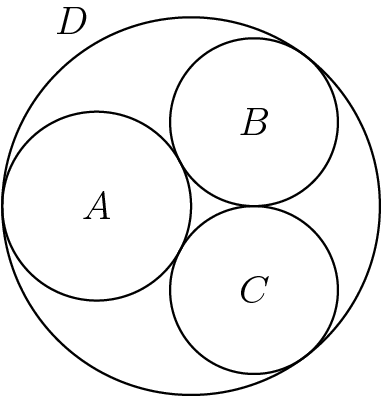
\includegraphics[height=7cm,page=1]{2021-07-24-figure-05}
\end{center}

\nopagebreak

\fbox{(A) $\dfrac{2}{3}$ \quad (B) $\dfrac{\sqrt{3}}{2}$ \quad (C) $\dfrac{7}{8}$ \quad (D) $\dfrac{8}{9}$ \quad (E) $\dfrac{1+\sqrt{3}}{3}$}

\begin{answer}
\bigskip
\begin{center}
  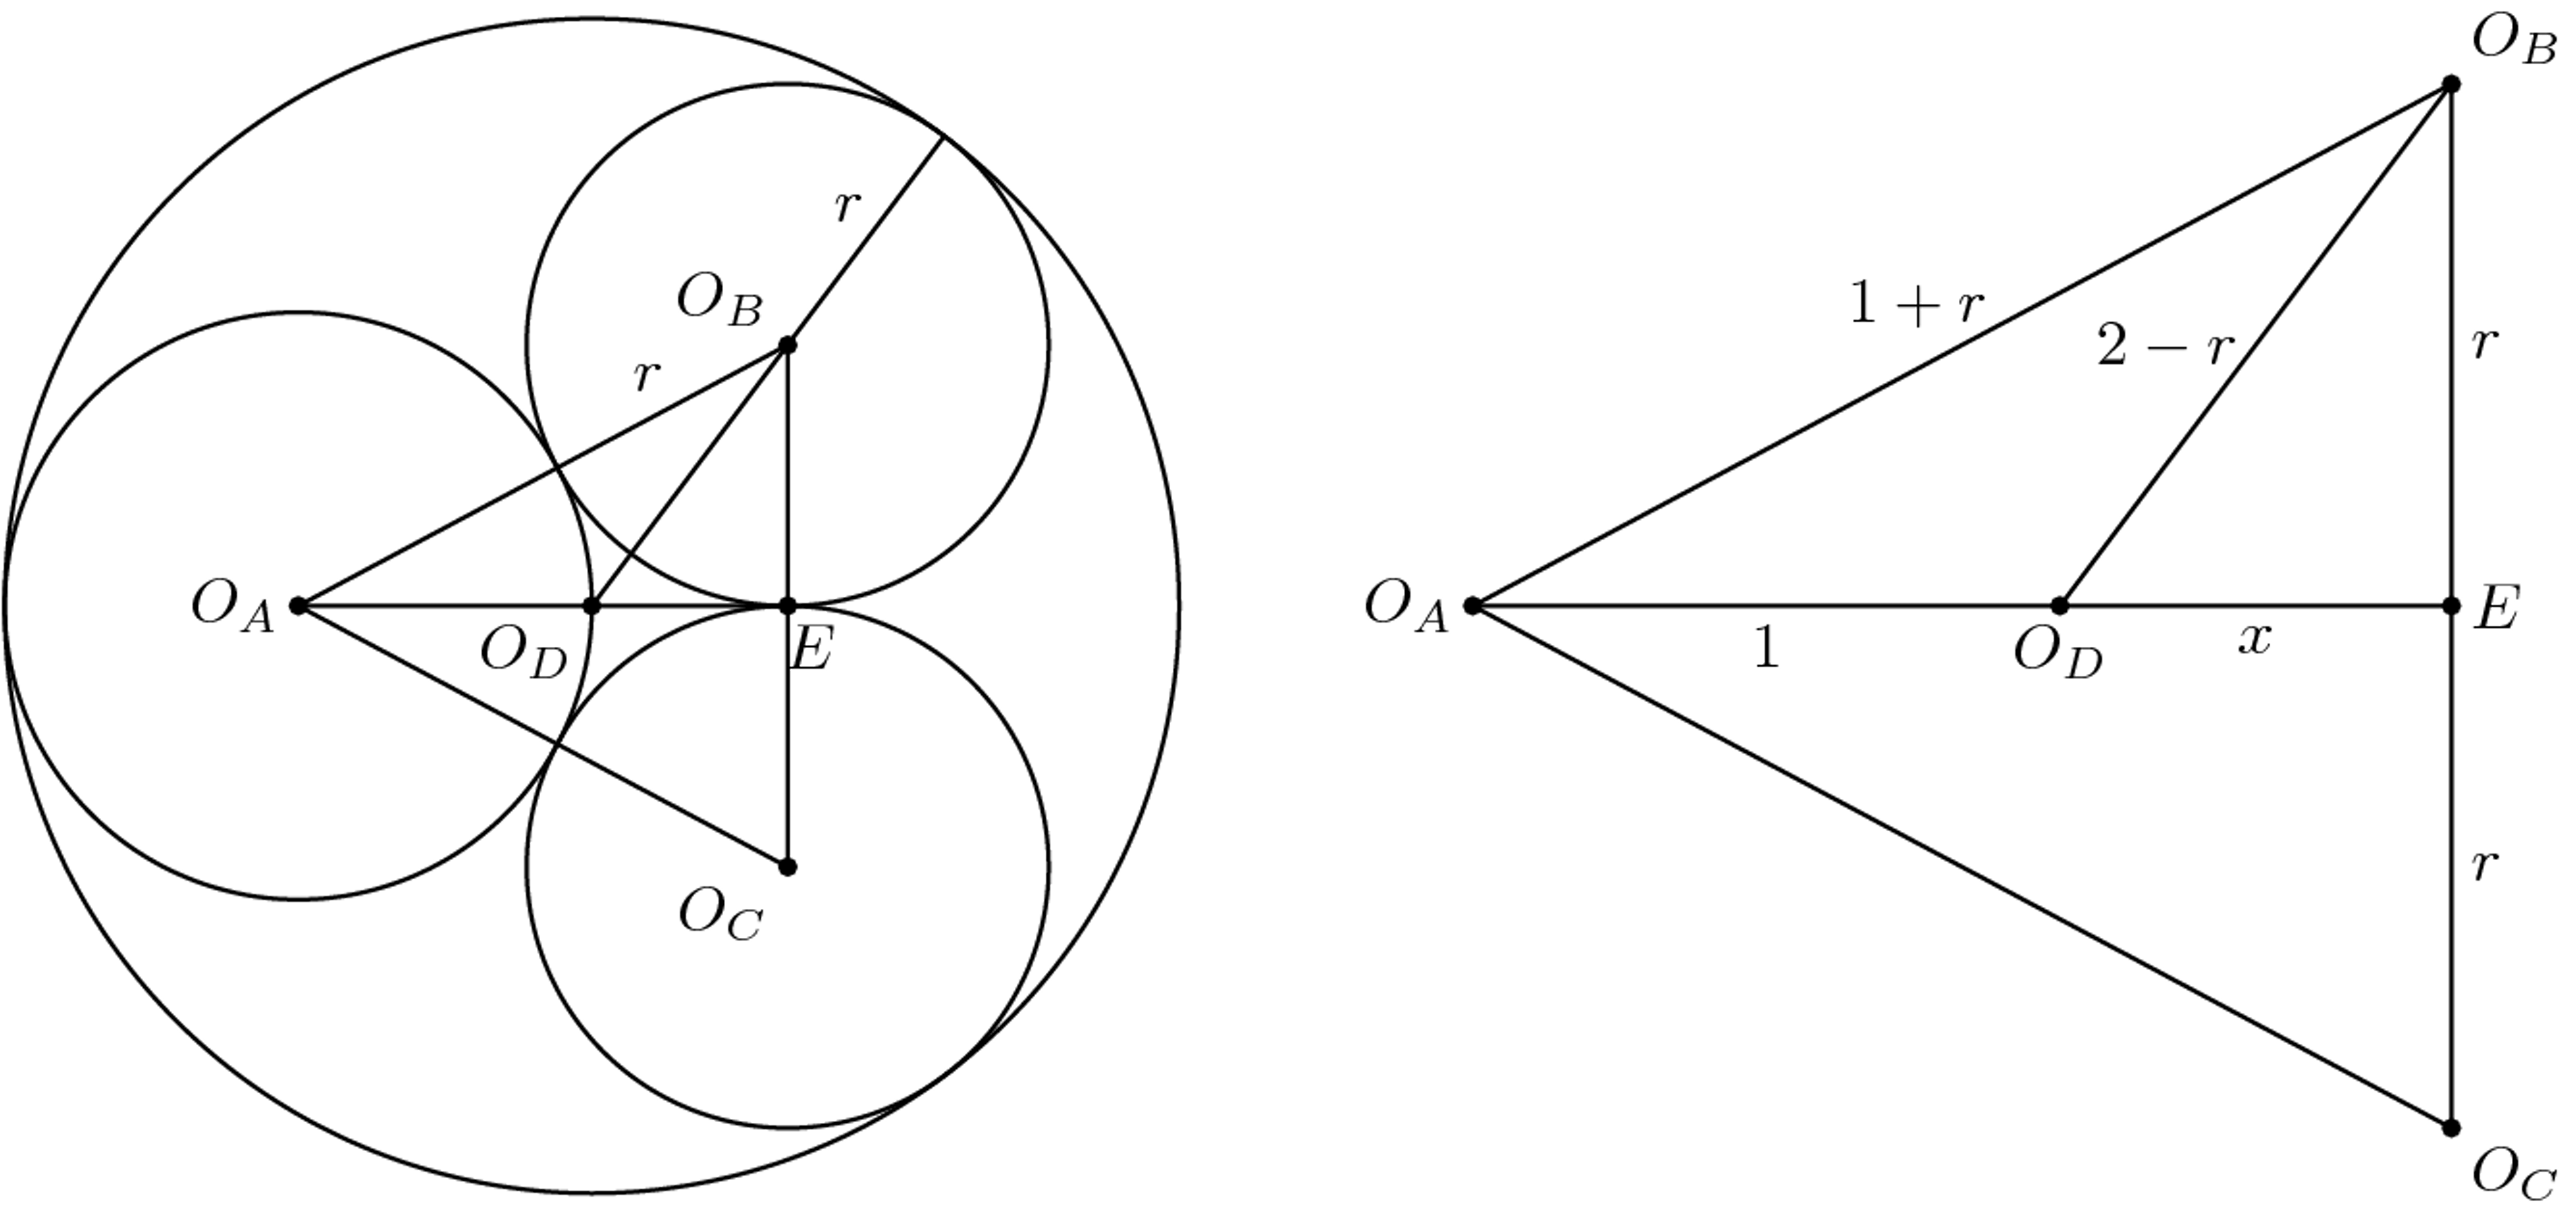
\includegraphics[height=8cm,page=1]{2021-07-24-figure-05b}
\end{center}
Since circle $A$ has radius $1$ and passes through the center of the large circle $D$, the radius of $D$ is $2$. Let $r$ denote the radius of circle $B$ (and of $C$). The triangle connecting the centers of the three inscribed circles is an isosceles triangle with lengths $1+r$, $1+r$, and $2r$. Refer to the triangle in the figure. Length $O_{B}O_{D}$ is $2-r$ since it is the radius of circle $O_{D}$ minus the radius of circle $O_{B}$. 

Triangles $O_{A}EO_{B}$ and $O_{D}EO_{B}$ both have a right angle at $E$ since $O_{A}E$ is the height of the isosceles triangle $O_{A}O_{B}O_{C}$ (and $E$ is the midpoint of the base $O_{B}O_{C}$). Let $x$ denote the distance $O_{D}E$ (see the second figure).

Apply the Pythagorean theorem to triangle $O_{D}EO_{C}$:
\begin{align*}
x^2 + r^2  
  & = (2-r)^2 \\
x & = 2\sqrt{1-r}
\end{align*}

Apply the Pythagorean theorem to triangle $O_{A}EO_{B}$:
\begin{align*}
r^2 + (1+x)^2  
  & = (1+r)^2 \\
r^2 + \left(1+2\sqrt{1-r}\right)^2 
  & = (1+r)^2 \\
r^2 + 1 + 4\sqrt{1-r} + 4(1-r)
  & = 1 + 2r + r^2 \\
4\sqrt{1-r} 
  & = 2r - 4(1-r) \\
\sqrt{1-r} 
  & = \frac{6r- 4}{4} \\
1-r 
  & = \left(\frac{3r}{2}-1\right)^2 \\
\frac{9r^2}{4} -3r + r
 & = 0 \\
r & = \frac{8}{9} 
\end{align*}
\begin{empheq}[box={\mathbox[colback=white]}]{equation*}
   \text{radius of circle B}~ = \frac{8}{9}
\end{empheq} 
\end{answer}
%%%%%%%%%%%%%%%%%%%%%%%%%%%%%%%%%%%%%%%%%%%%%%%%%%%%%%%%%%%%%%%%%%%%%%%%

\iftoggle{showAnswers}{\newpage}

%%%%%%%%%%%%%%%%%%%%%%%%%%%%%%%%%%%%%%%%%%%%%%%%%%%%%%%%%%%%%%%%%%%%%%%%
\subsection*{6.}

\nopagebreak

Let $\overline{AB}$ be a diameter of a circle and $C$ be a point on $\overline{AB}$ with $2 \cdot AC = BC$. Let $D$ and $E$ be points on the circle such that $\overline{DC} \perp \overline{AB}$ and $\overline{DE}$ is a second diameter. What is the ratio of the area of triangle $DCE$ to the area of triangle $ABD$?

\nopagebreak

\begin{center}
  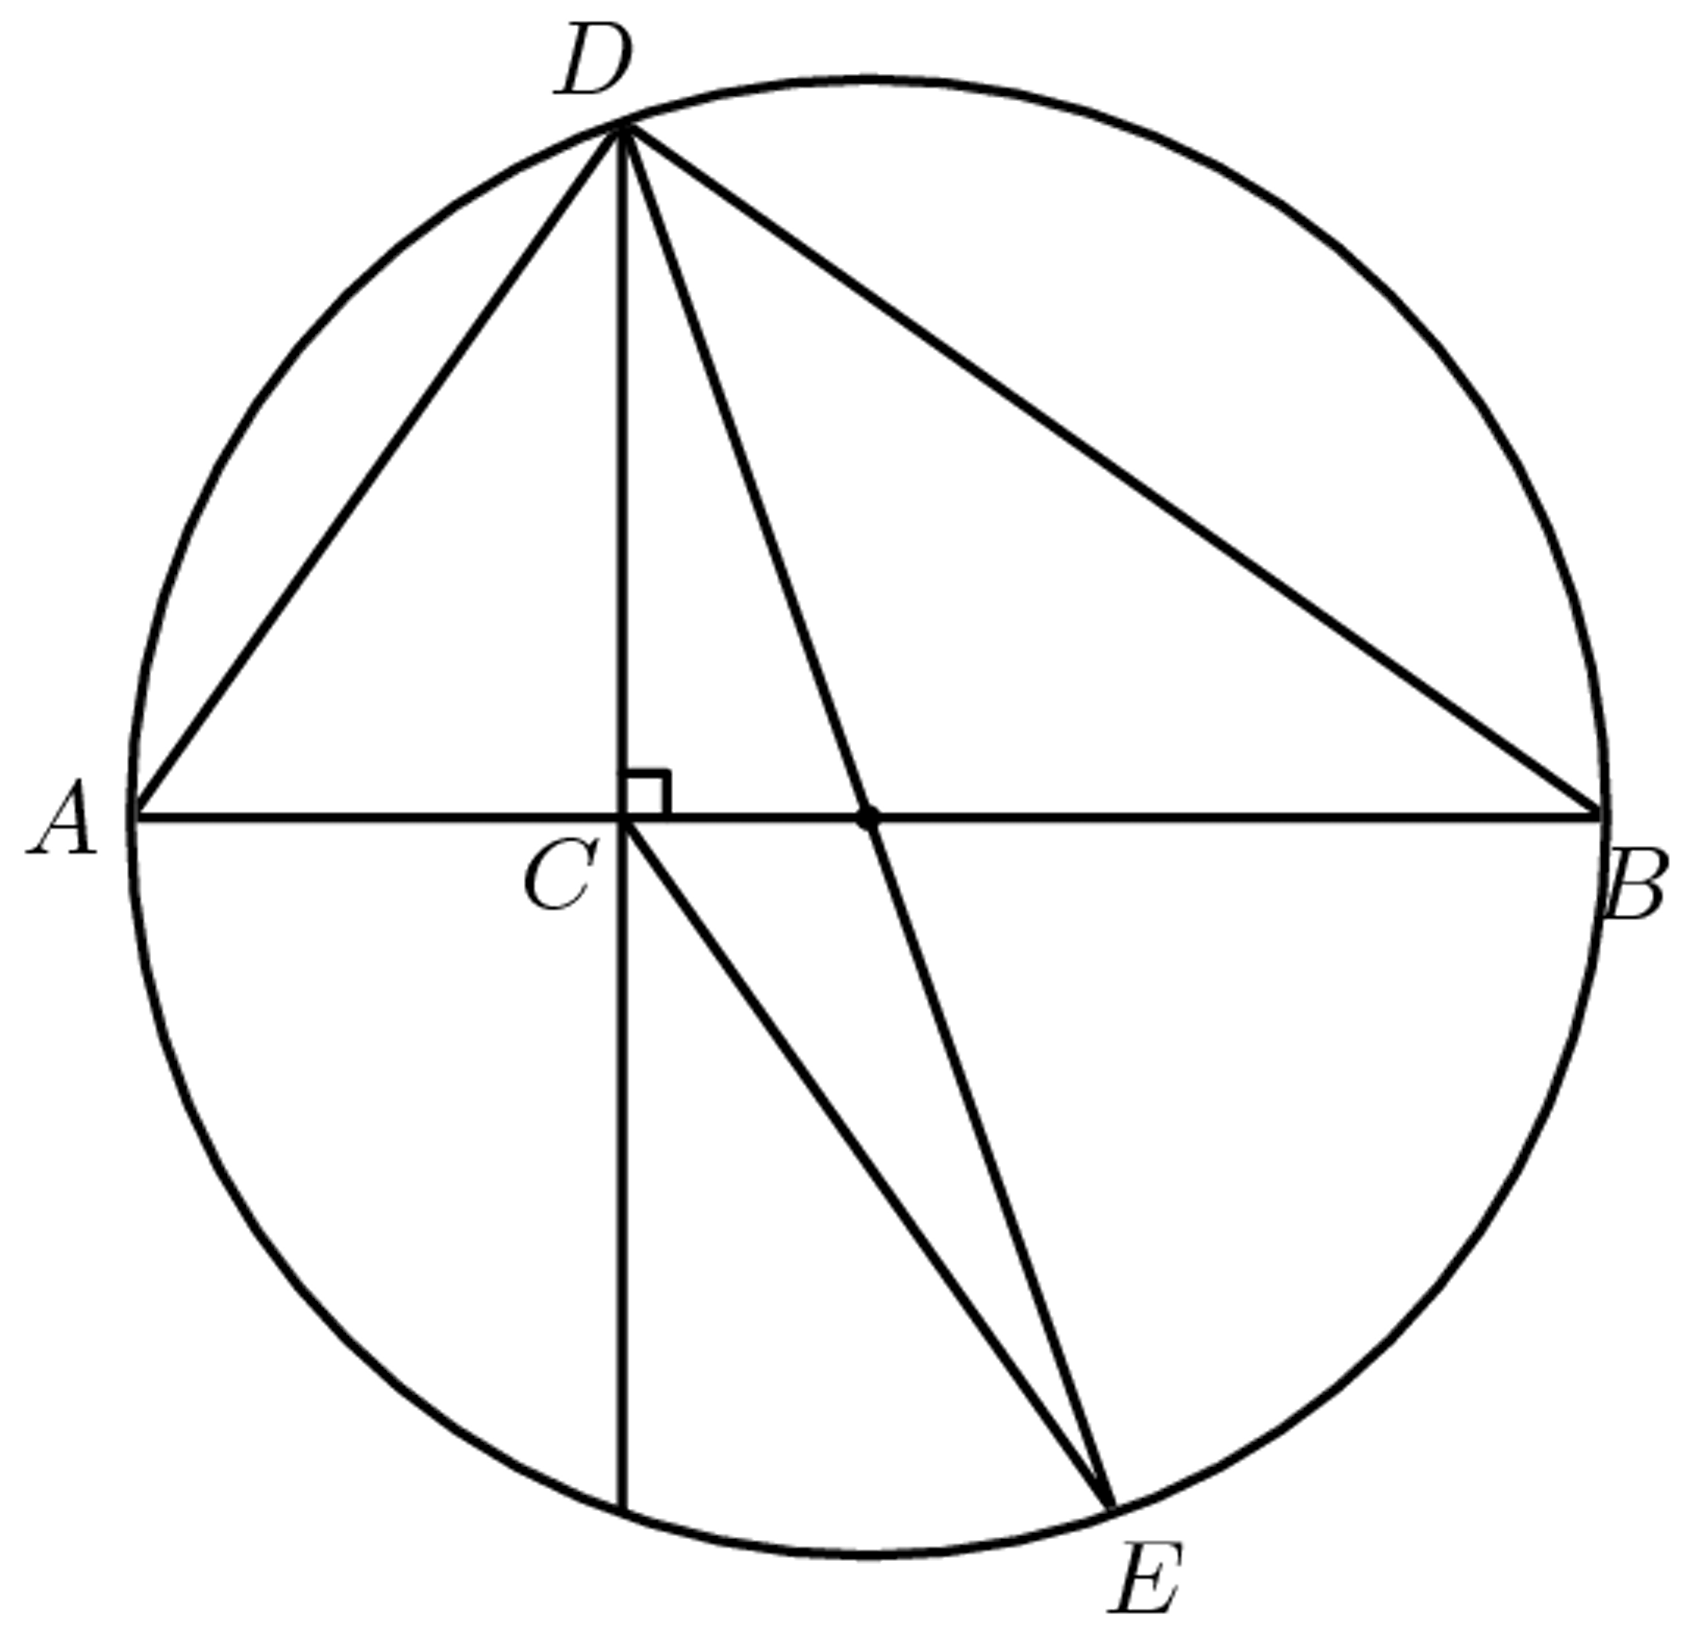
\includegraphics[height=8cm,page=1]{2021-07-24-figure-06}
\end{center}

\nopagebreak

\fbox{(A) $\dfrac{1}{6}$ \quad (B) $\dfrac{1}{4}$ \quad (C) $\dfrac{1}{3}$ \quad (D) $\dfrac{1}{2}$ \quad (E) $\dfrac{2}{3}$}

\begin{answer}
Let $O$ denote the center of the circle. We have
\begin{align*}
2 AC = BC 
\implies 
3 AC = AB
\end{align*}
Since $O$ is the midpoint of $AB$, we have
\begin{align*}
\frac{3}{2}AC = AO 
\implies 
CO = \frac{1}{3} AO 
\implies 
CO = \frac{1}{6} AB
\end{align*}
Since $O$ is the midpoint of $DE$, we have
\begin{align*}
[\triangle DCE] 
  & = 2 \, [\triangle DCO] \\
  & = 2 \cdot \, \frac{1}{6} [\triangle ABD] \\
  & = \frac{1}{3} \, [\triangle ABD]
\end{align*}
\begin{empheq}[box={\mathbox[colback=white]}]{equation*}
  \frac{[\triangle DCE]}{[\triangle ABD]}
    = \frac{1}{3}
\end{empheq} 
\end{answer}
%%%%%%%%%%%%%%%%%%%%%%%%%%%%%%%%%%%%%%%%%%%%%%%%%%%%%%%%%%%%%%%%%%%%%%%%

\iftoggle{showAnswers}{\newpage}

%%%%%%%%%%%%%%%%%%%%%%%%%%%%%%%%%%%%%%%%%%%%%%%%%%%%%%%%%%%%%%%%%%%%%%%%
\subsection*{7.}

\nopagebreak

Riders on a Ferris wheel travel in a circle in a vertical plane. A particular wheel has radius $20$ feet and revolves at the constant rate of one revolution per minute. How many seconds does it take a rider to travel from the bottom of the wheel to a point $10$ vertical feet above the bottom?

\nopagebreak

\fbox{(A) $5$ \quad (B) $6$ \quad (C) $7.5$ \quad (D) $10$ \quad (E) $15$}

\begin{answer}
Let $O$ denote the center of the Ferris wheel and $C$ a point located $10$ feet above the bottom. Let $B$ denote the projection of $C$ onto the vertical line $OA$. 
\bigskip
\begin{center}
  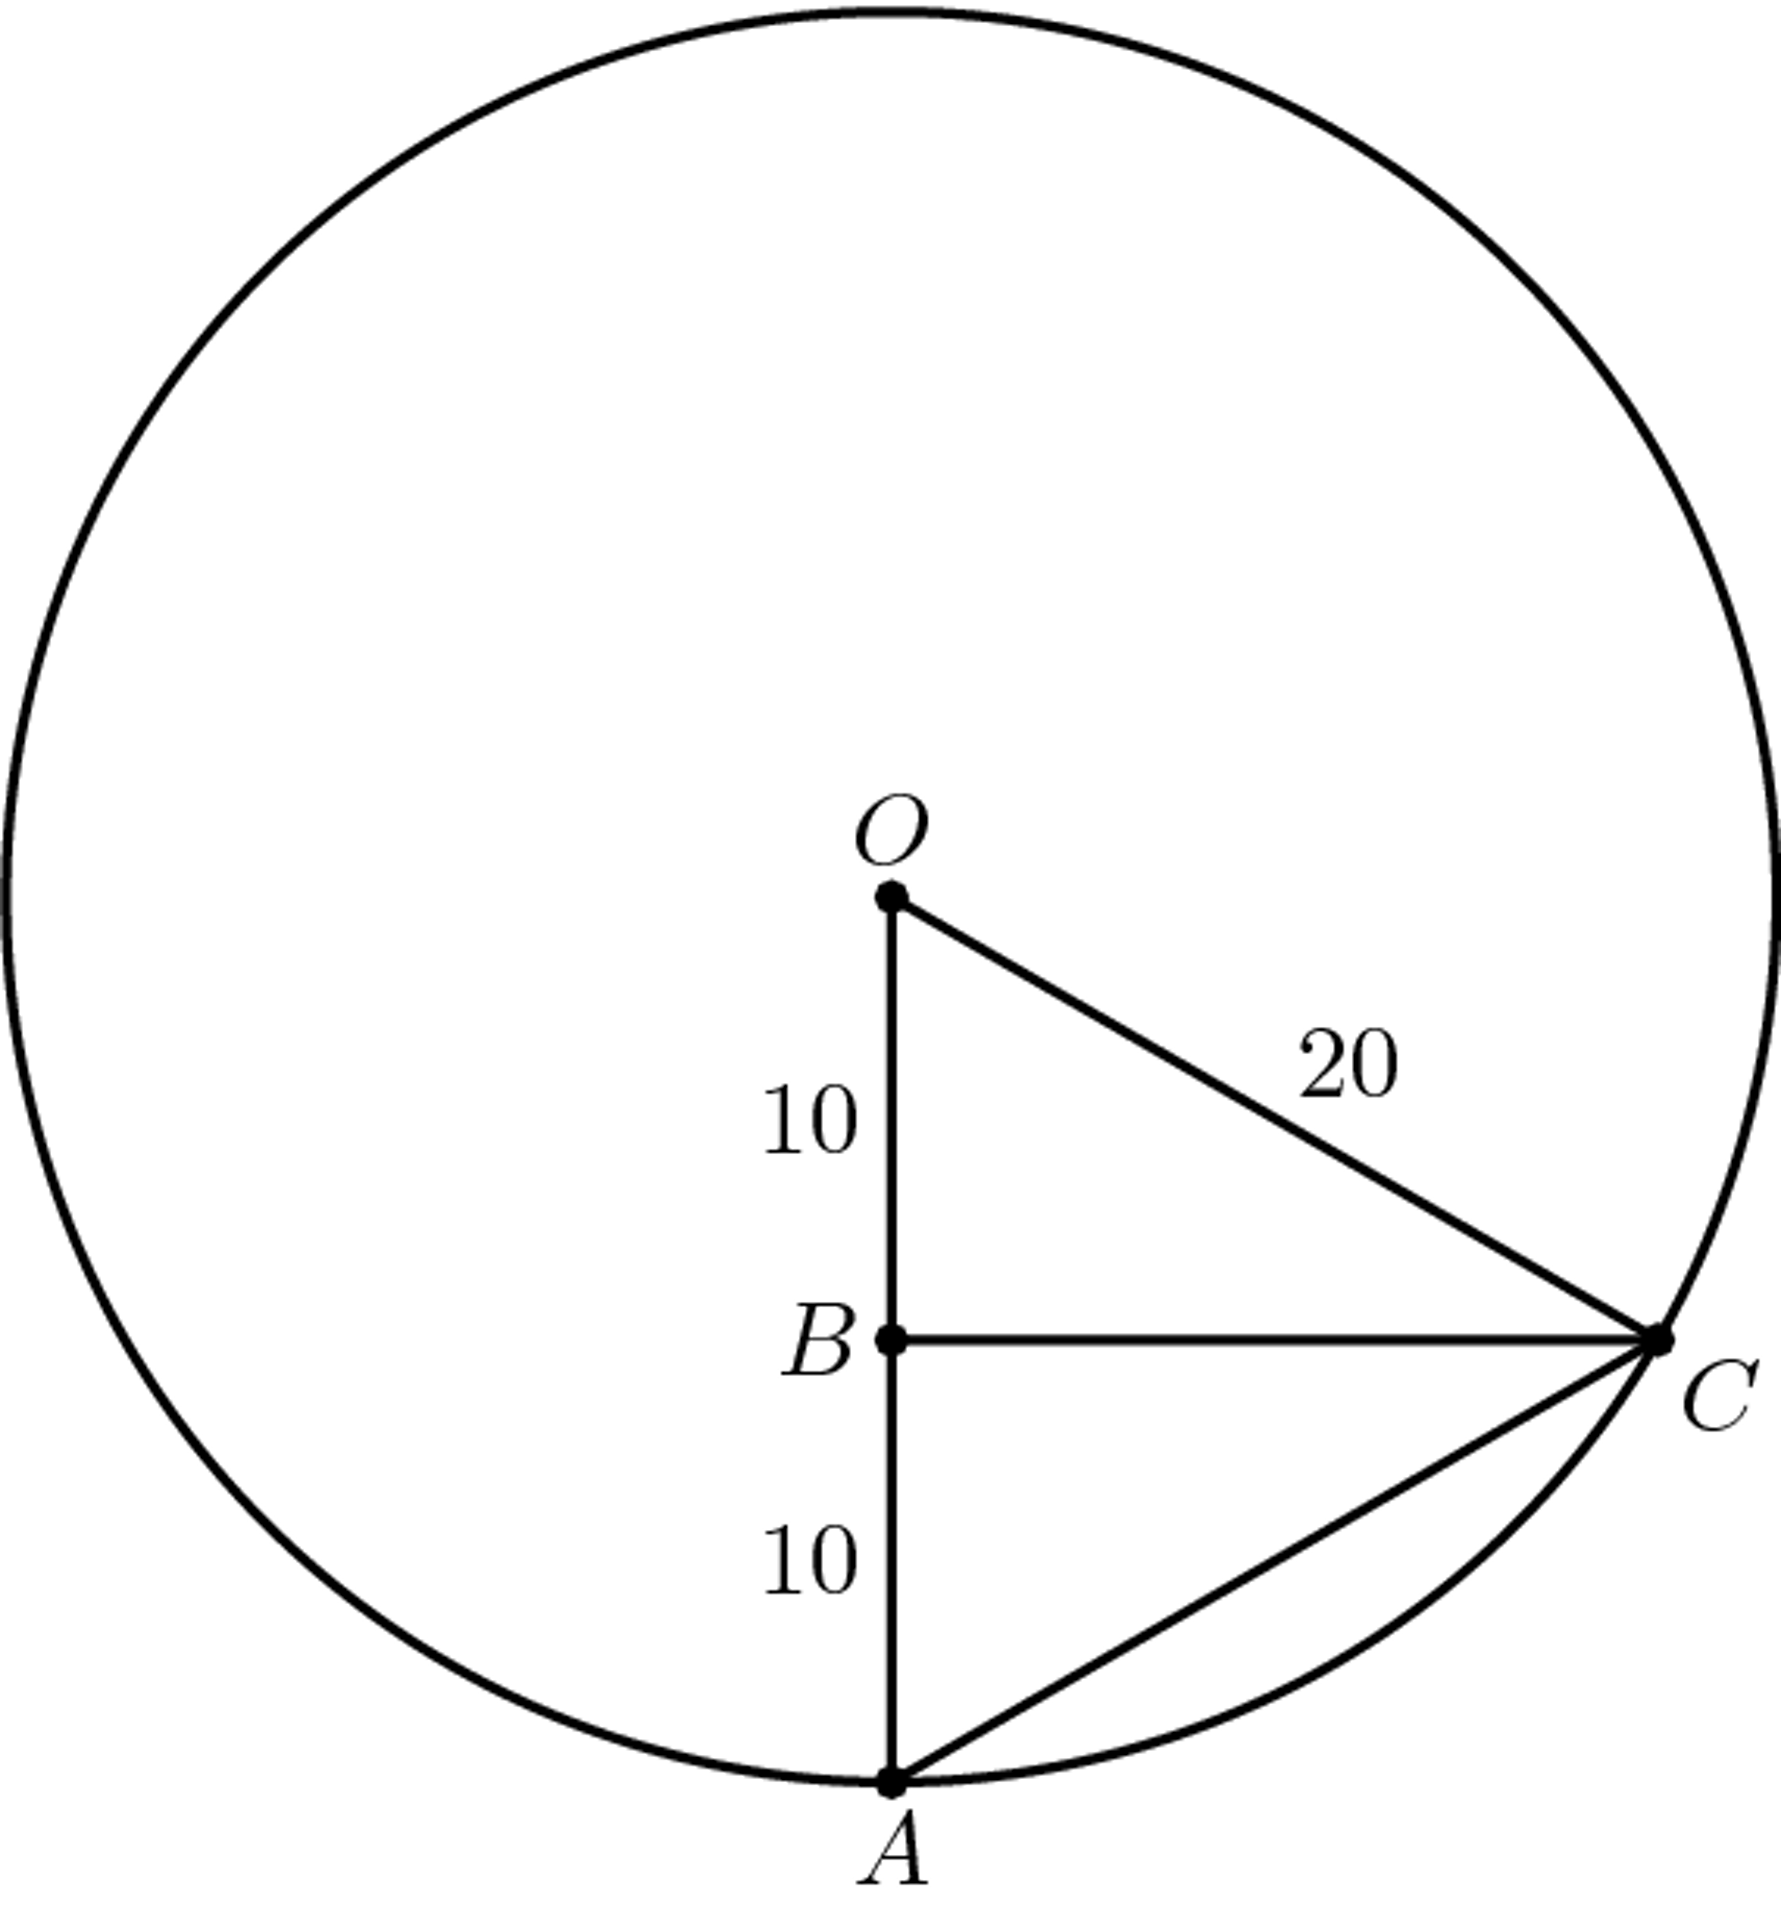
\includegraphics[height=8cm,page=1]{2021-07-24-figure-07}
\end{center}
\bigskip
At a distance of $10$ feet, $BA=10$, and so $B$ is the midpoint of $OA$, implying that triangle $\triangle OAC$ is equilateral with side length $20$, and $\angle BOC = 60^\circ$. At point $C$, the Ferris wheel has completed $\dfrac{60}{360}=\dfrac{1}{6}$ of a revolution in one-sixth of a minute, or $10$ seconds. 
\begin{empheq}[box={\mathbox[colback=white]}]{equation*}
    10 ~\text{seconds}
\end{empheq} 
\end{answer}
%%%%%%%%%%%%%%%%%%%%%%%%%%%%%%%%%%%%%%%%%%%%%%%%%%%%%%%%%%%%%%%%%%%%%%%%

\iftoggle{showAnswers}{\newpage}

%%%%%%%%%%%%%%%%%%%%%%%%%%%%%%%%%%%%%%%%%%%%%%%%%%%%%%%%%%%%%%%%%%%%%%%%
\subsection*{8.}

\nopagebreak

In triangle $ABC$ we have $AB = 7$, $AC = 8$, and $BC = 9$. Point $D$ is on the circumscribed circle of the triangle so that $\overline{AD}$ bisects $\angle BAC$. What is the value of $AD/CD$?

\nopagebreak

\fbox{(A) $\dfrac{9}{8}$ \quad (B) $\dfrac{5}{3}$ \quad (C) $2$ \quad (D) $\dfrac{17}{7}$ \quad (E) $\dfrac{5}{2}$}

\begin{answer}
\begin{center}
  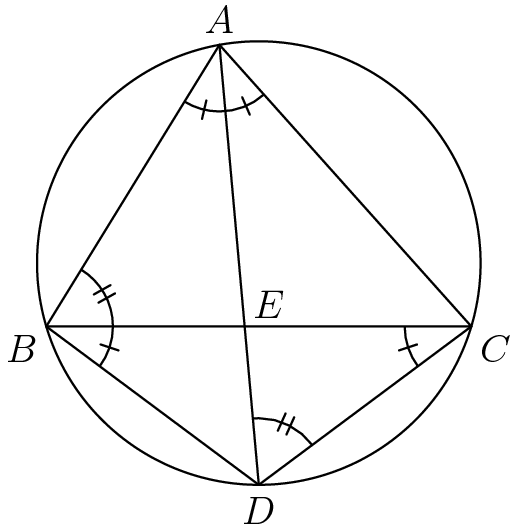
\includegraphics[height=8cm,page=1]{2021-07-24-figure-08}
\end{center}
\bigskip
Since $AE$ bisects $\angle BAC$, $E$ is the midpoint of $BC$, implying $BD=CD$. Therefore triangles $\triangle ABE$ and $\triangle ADC$ are similar, implying
\begin{align*}
\frac{AD}{AB} = \frac{CD}{BE}
\implies
\frac{AD}{CD} = \frac{7}{BE}
\end{align*}
To find $BE$, consider triangles $\triangle ABE$ and $\triangle ACE$. Since $AE$ bisects the angle, the sines are equal:
\begin{align*}
\frac{BE}{AB} = \frac{CE}{AC}
\implies
\frac{BE}{7} = \frac{9-BE}{8}
\implies
BE = \frac{21}{5}
\end{align*}
Substituting $BE$ back gives
\begin{align*}
\frac{AD}{CD} 
  = \frac{7}{\dfrac{21}{5}}
  = \frac{5}{3}
\end{align*}
\begin{empheq}[box={\mathbox[colback=white]}]{equation*}
    \frac{AD}{CD} = \frac{5}{3}
\end{empheq} 
\end{answer}
%%%%%%%%%%%%%%%%%%%%%%%%%%%%%%%%%%%%%%%%%%%%%%%%%%%%%%%%%%%%%%%%%%%%%%%%

\iftoggle{showAnswers}{\newpage}

%%%%%%%%%%%%%%%%%%%%%%%%%%%%%%%%%%%%%%%%%%%%%%%%%%%%%%%%%%%%%%%%%%%%%%%%
\subsection*{9.}

\nopagebreak

Circles with centers $O$ and $P$ have radii $2$ and $4$, respectively, and are externally tangent. Points $A$ and $B$ are on the circle centered at $O$, and points $C$ and $D$ are on the circle centered at $P$, such that $\overline{AD}$ and $\overline{BC}$ are common external tangents to the circles. What is the area of hexagon $AOBCPD$?

\nopagebreak

\begin{center}
  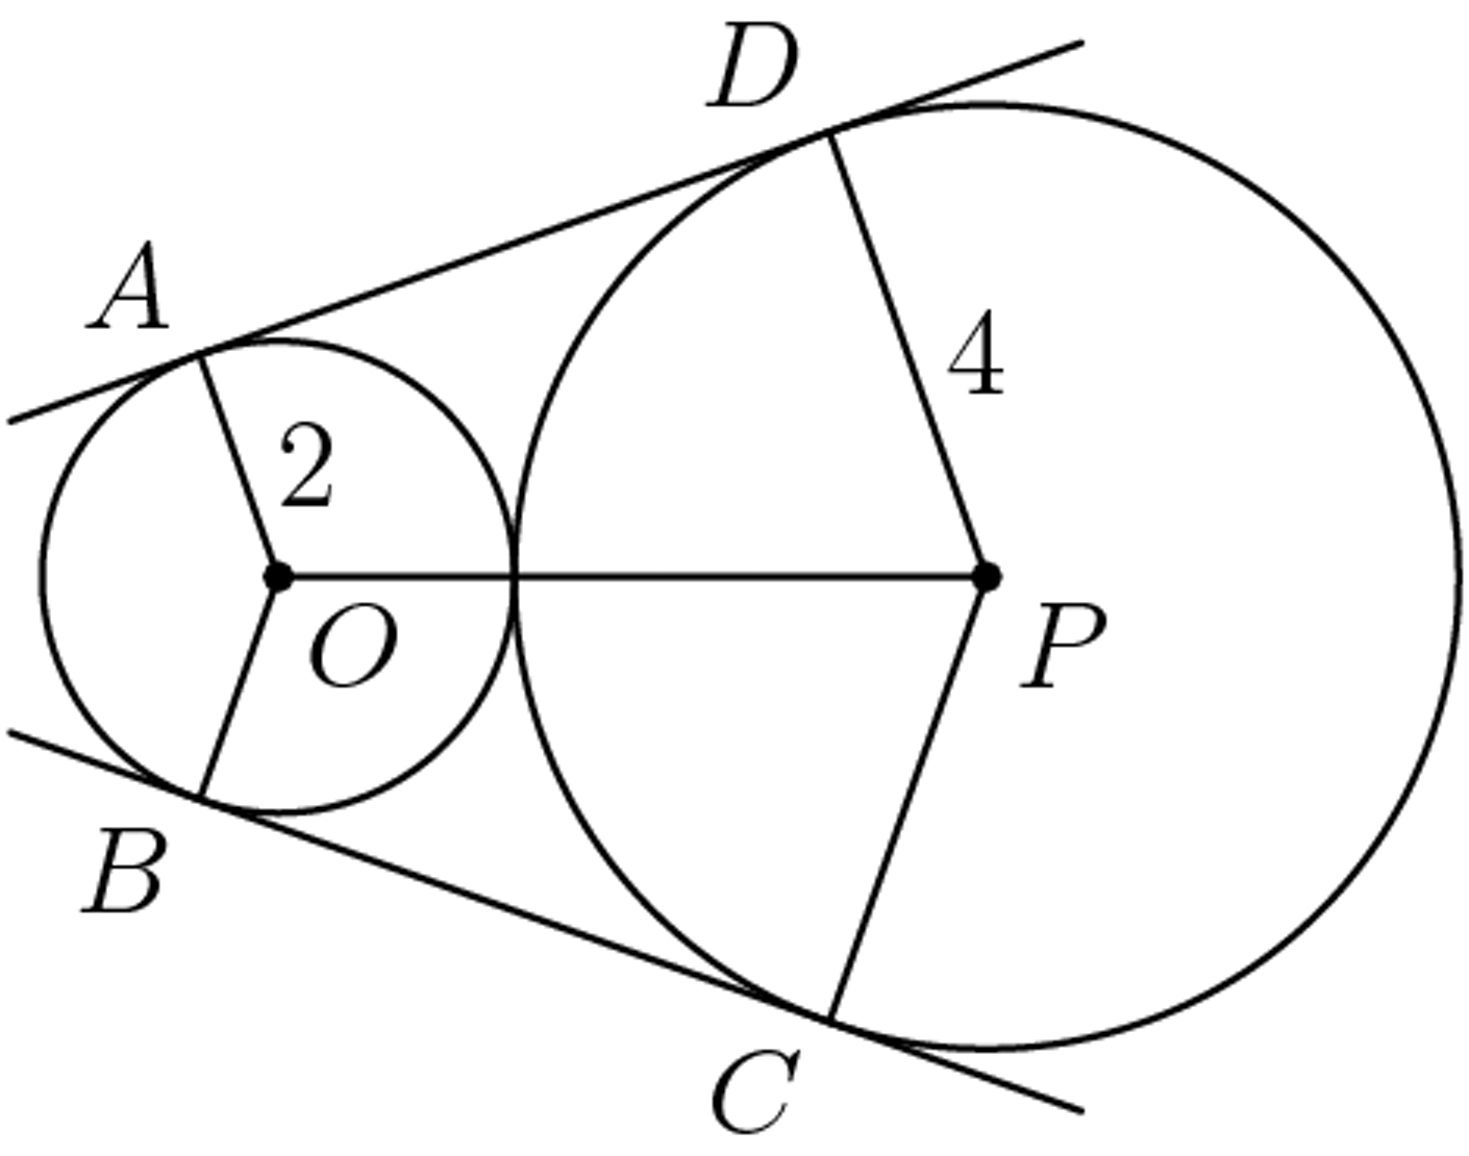
\includegraphics[height=5cm,page=1]{2021-07-24-figure-09}
\end{center}

\nopagebreak

\fbox{(A) $18\sqrt{3}$ \quad (B) $24\sqrt{2}$ \quad (C) $36$ \quad (D) $24\sqrt{3}$ \quad (E) $32\sqrt{2}$}

\begin{answer}
Project point $O$ onto $DP$ and call the projected point $O^{\prime}$. Angles $\angle OAD$ and $\angle ADP$ are both right angles since $AD$ is tangent to both circles. Since quadrilateral $AOO^{\prime}D$ has three right angles, it must be a rectangle and $O^{\prime}$ is therefore the midpoint of $DP$, so that $O^{\prime}D=O^{\prime}P=2$. We also know that $OP=4+2=6$. The Pythagorean theorem applied to $OO^{\prime}P$ gives 
\begin{align*}
OO^{\prime} = \sqrt{6^2-2^2} = 4\sqrt{2}
\end{align*}
The area of the trapezoid $AOPD$ is thus:
\begin{align*}
2 \cdot 4\sqrt{2} 
  + \frac{1}{2} \cdot 2 \cdot 4\sqrt{2}
  = 12 \sqrt{2}
\end{align*}
And so the area of the entire hexagon is:
\begin{empheq}[box={\mathbox[colback=white]}]{equation*}
    24 \sqrt{2}
\end{empheq} 
\end{answer}
%%%%%%%%%%%%%%%%%%%%%%%%%%%%%%%%%%%%%%%%%%%%%%%%%%%%%%%%%%%%%%%%%%%%%%%%

\iftoggle{showAnswers}{\newpage}

%%%%%%%%%%%%%%%%%%%%%%%%%%%%%%%%%%%%%%%%%%%%%%%%%%%%%%%%%%%%%%%%%%%%%%%%
\subsection*{10.}

\nopagebreak

A circle of radius 1 is internally tangent to two circles of radius 2 at points $A$ and $B$, where $AB$ is a diameter of the smaller circle. What is the area of the region, shaded in the figure, that is outside the smaller circle and inside each of the two larger circles?

\nopagebreak

\begin{center}
  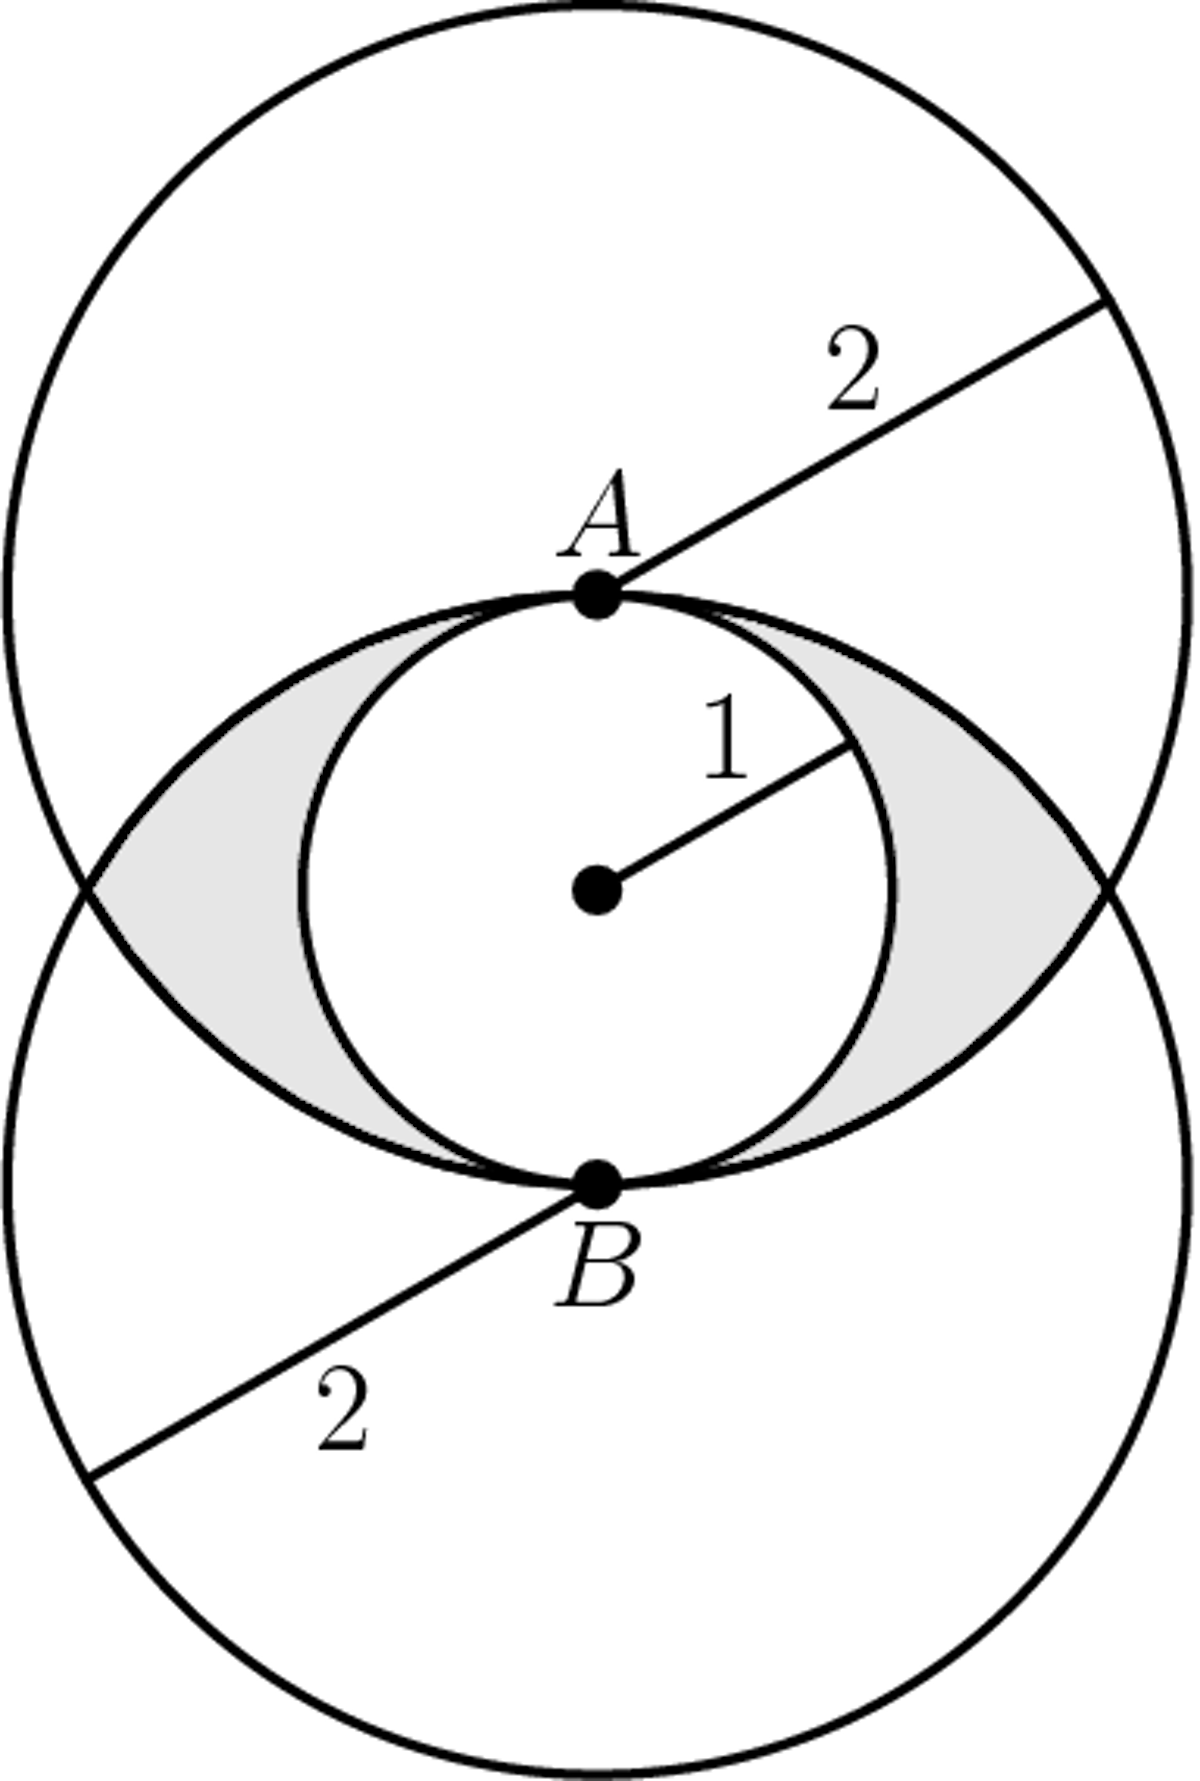
\includegraphics[height=9cm,page=1]{2021-07-24-figure-10}
\end{center}

\nopagebreak

\fbox{(A) $\dfrac{5}{3}\pi-3\sqrt{2}$ \quad (B) $\dfrac{5}{3}\pi-2\sqrt{3}$ \quad (C) $\dfrac{8}{3}\pi-3\sqrt{3}$ \quad (D) $\dfrac{8}{3}\pi-3\sqrt{2}$ \quad (E) $\dfrac{8}{3}\pi-2\sqrt{3}$}

\begin{answer}
Connect $A$ and $B$ with the points $C$ and $D$ defined by the intersection of the circles, as shown in the figure. 
\begin{center}
  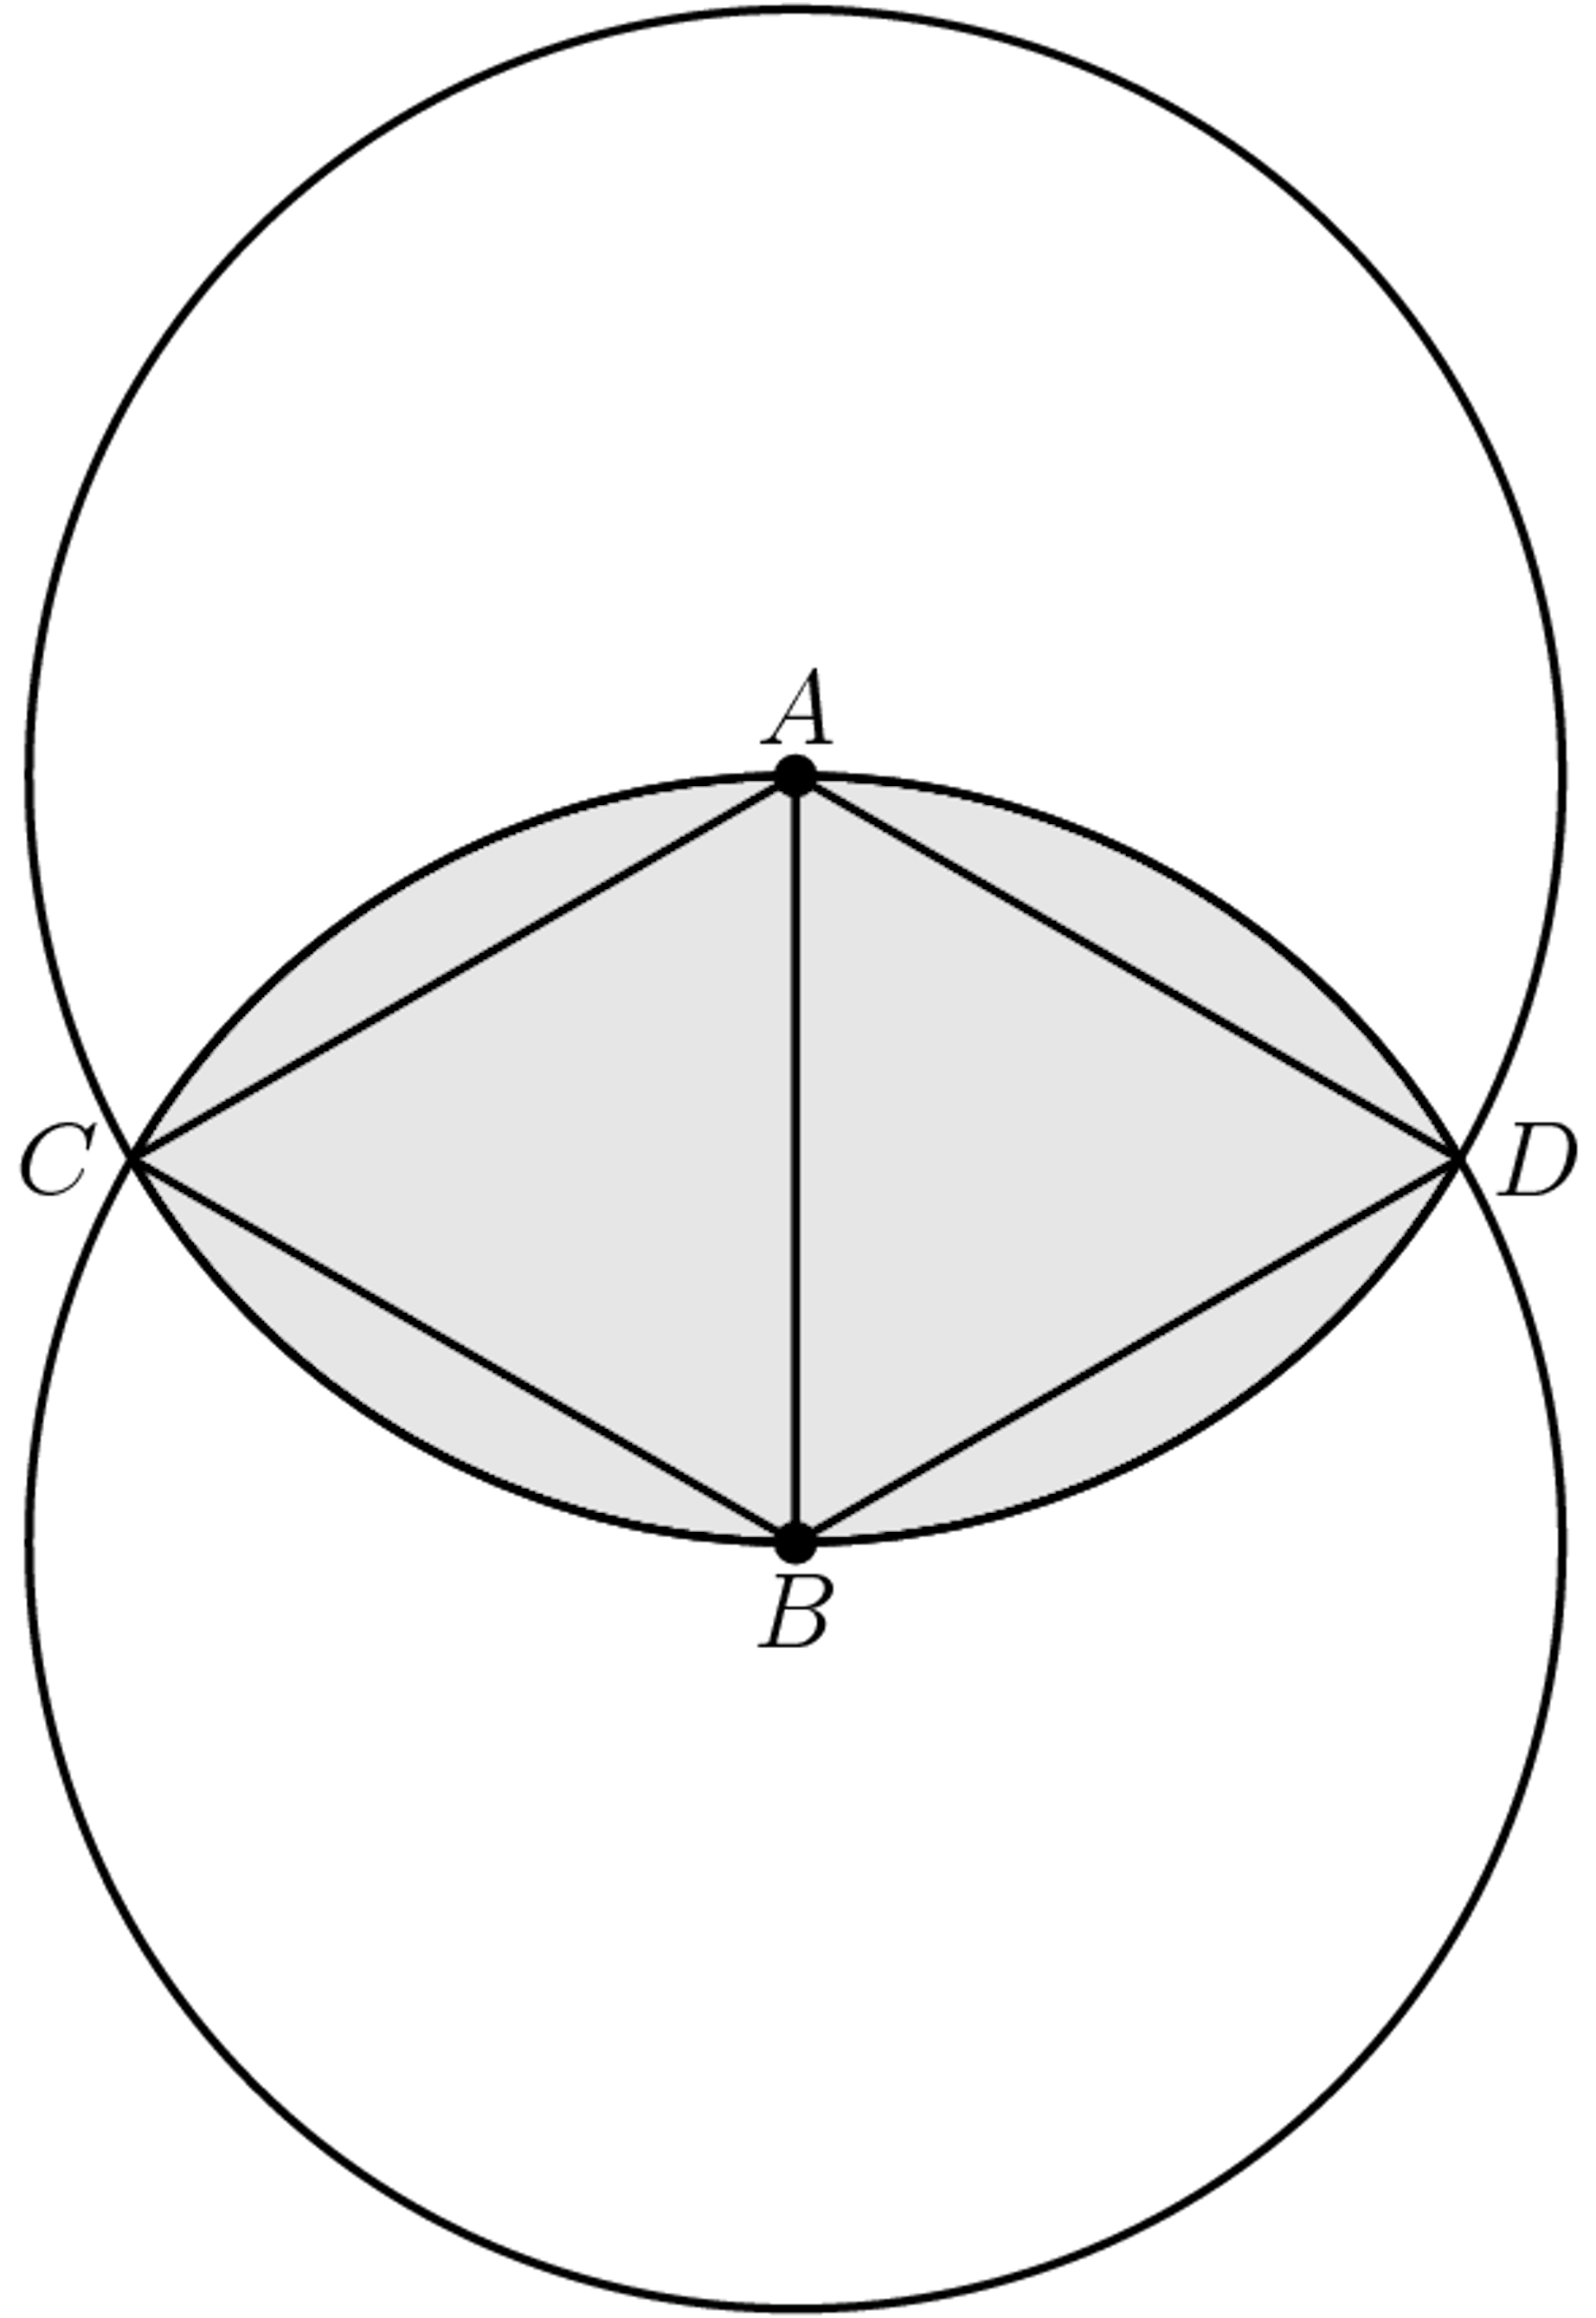
\includegraphics[height=9cm,page=1]{2021-07-24-figure-10b}
\end{center}
\bigskip
Triangle $\triangle ABC$ is equilateral, with side length $AB=BC=AC=2$ and all three angles of measure $60^\circ=\pi/3$. Thus, the sector associated with $\angle ABC$ covers a fraction $\dfrac{\pi/3}{2\pi}=\dfrac{1}{6}$ of the area of a circle of radius $2$, or $\dfrac{2\pi}{3}$. Likewise for sectors $ABD$, $CAB$, and $BAD$. If we add the area of the four sectors, however, we double-count the two equilateral triangles. Each of these triangles has area $\dfrac{\sqrt{3}}{4}\cdot2^2=\sqrt{3}$. The area of the intersection of the two circles (shaded in the second figure) is therefore:
\begin{align*}
4 \cdot \frac{2\pi}{3} - 2 \cdot \sqrt{3}
  & = \frac{8}{3} \pi - 2\sqrt{3}
\end{align*}
Now subtract the area of the non-shaded circle:
\begin{align*}
\frac{8}{3} \pi - 2\sqrt{3} - \pi 
  = \frac{5}{3} \pi - 2\sqrt{3}
\end{align*}
\begin{empheq}[box={\mathbox[colback=white]}]{equation*}
    \frac{5}{3} \pi - 2\sqrt{3}
\end{empheq} 
\end{answer}
%%%%%%%%%%%%%%%%%%%%%%%%%%%%%%%%%%%%%%%%%%%%%%%%%%%%%%%%%%%%%%%%%%%%%%%%

\iftoggle{showAnswers}{\newpage}

\end{document}
